\chapter{Grover's search algorithm}\label{ch:grover}

Grover's algorithm \cite{Grover1996} solves the problem of searching an unordered database, that is, a list of $N$ elements without any index or sorting. Classically, there is no better strategy than
checking the elements one by one. On average, $N/2$ checks are needed to find the desired element with probability $1/2$, so the cost grows as $N$. Grover's quantum algorithm needs only of the order of
$\sqrt N$ queries: a \emph{quadratic} speed-up. Since many problems (e.g.\ NP problems) can be phrased as a search for an input that satisfies an efficiently checkable condition, the algorithm is very general.

\section{The oracle}
The element to find, $w$, is characterized by the function
\begin{equation}
  f_w(x)=\begin{cases}0,&x\neq w,\\1,&x=w.\end{cases}
\end{equation}
This function is implemented as a quantum oracle acting on an $n$-qubit register $\ket x$ (with $N=2^n$) and one additional qubit $\ket y$: $U\ket x\ket y=\ket x\ket{y\oplus f_w(x)}$, where $\oplus$ denotes
addition modulo 2, $a\oplus b=(a+b)\bmod2$, so that $1\oplus1=0$. For $x=w$ the oracle flips the qubit $\ket y$: $\ket w\ket0\to\ket w\ket1$, $\ket w\ket1\to\ket w\ket0$, while for $x\neq w$ nothing changes.

The best choice for the additional qubit is $\ket y=\ket-=(\ket0-\ket1)/\sqrt2$. Flipping this qubit only changes its sign (phase kickback, \cref{eq:kickback}), so we can forget it and describe the oracle as the operator
\begin{equation}
  O:\ket x\to(-1)^{f_w(x)}\ket x,\qquad O=I-2\proj w .
\end{equation}
It is important to understand what the oracle is. It does not ``know'' the answer; it \emph{recognizes} it. For a search for the solution of a problem (e.g.\ a satisfying assignment of a Boolean formula),
$O$ is a circuit that evaluates the condition, which is usually easy, while finding the input that satisfies it is hard.

\section{The algorithm}
The register is first prepared in an equal superposition of all $N$ basis states by applying a Hadamard gate to each qubit of $\ket{0\dots0}$:
\begin{equation}
  \ket\psi=\frac1{\sqrt N}\sum_{x=0}^{N-1}\ket x=\frac1{\sqrt N}\left(\ket{0\dots00}+\ket{0\dots01}+\dots+\ket{1\dots11}\right).
\end{equation}
The \emph{Grover iteration} $G$ is then repeated several times. It consists of four steps:
\begin{enumerate}
  \item apply the oracle $O$;
  \item apply Hadamard gates to all qubits;
  \item apply a conditional phase shift, which changes the sign of every basis state except $\ket0$: $\ket x\to-(-1)^{\delta_{x0}}\ket x$, where $\delta_{x0}$ is the Kronecker delta. This operation is $2\proj0-I$;
  \item apply Hadamard gates to all qubits again.
\end{enumerate}
Since the Hadamard transform maps $\ket0$ onto $\ket\psi$ and is its own inverse, steps 2--4 together give
\begin{equation}
  H^{\otimes n}(2\proj0-I)H^{\otimes n}=2H^{\otimes n}\proj0H^{\otimes n}-H^{\otimes n}H^{\otimes n}=2\proj\psi-I.
\end{equation}
The Grover iteration is therefore
\begin{equation}\label{eq:grover}
  G=\left(2\proj\psi-I\right)O.
\end{equation}
The operator $D=2\proj\psi-I$ is called the \emph{diffusion} operator, or ``inversion about the mean'': for $\ket\phi=\sum_xa_x\ket x$ with mean amplitude $\bar a=\frac1N\sum_xa_x$,
$D\ket\phi=\sum_x(2\bar a-a_x)\ket x$. Each amplitude is reflected about the mean. After the oracle has flipped the sign of the solution, its amplitude is far below the mean, and the reflection
makes it grow; this is the intuition of Grover's original paper.

\section{Geometric interpretation}
Let us generalize slightly and assume that $M$ of the $N$ elements are solutions ($1\le M<N$). We define two normalized states, the superpositions of the non-solutions and of the solutions:
\begin{equation}
  \ket\alpha=\frac1{\sqrt{N-M}}\sum_{x\notin\text{sol.}}\ket x,\qquad\ket\beta=\frac1{\sqrt M}\sum_{x\in\text{sol.}}\ket x.
\end{equation}
The initial state lies in the plane spanned by $\ket\alpha$ and $\ket\beta$:
\begin{equation}
  \ket\psi=\sqrt{\frac{N-M}N}\ket\alpha+\sqrt{\frac MN}\ket\beta=\cos\frac\theta2\ket\alpha+\sin\frac\theta2\ket\beta,\qquad\sin\frac\theta2=\sqrt{\frac MN}.
\end{equation}
The oracle changes the sign of all the basis states that are solutions: $O\ket\alpha=\ket\alpha$, $O\ket\beta=-\ket\beta$. Both $O$ and $D$ map the plane onto itself, so the whole evolution stays in
this two-dimensional plane, however large $N$ is. In the basis $(\ket\alpha,\ket\beta)$,
\begin{equation}
  O=\begin{pmatrix}1&0\\0&-1\end{pmatrix},\qquad
  D=2\begin{pmatrix}\cos\frac\theta2\\ \sin\frac\theta2\end{pmatrix}\begin{pmatrix}\cos\frac\theta2&\sin\frac\theta2\end{pmatrix}-I=\begin{pmatrix}\cos\theta&\sin\theta\\ \sin\theta&-\cos\theta\end{pmatrix},
\end{equation}
\begin{equation}
  G=DO=\begin{pmatrix}\cos\theta&-\sin\theta\\ \sin\theta&\cos\theta\end{pmatrix}.
\end{equation}
In the $(\ket\alpha,\ket\beta)$ plane, $O$ is a reflection about $\ket\alpha$, and $D$ is a reflection about $\ket\psi$: it leaves the component along $\ket\psi$ unchanged and reverses the orthogonal component.
The product of two reflections is a rotation by twice the angle between the two mirrors. The angle between $\ket\alpha$ and $\ket\psi$ is $\theta/2$, so $G$ rotates the state by $\theta$ towards $\ket\beta$ (\cref{fig:grover}):
\begin{equation}
  G\ket\psi=\cos\frac{3\theta}2\ket\alpha+\sin\frac{3\theta}2\ket\beta,\qquad
  G^k\ket\psi=\cos\frac{(2k+1)\theta}2\ket\alpha+\sin\frac{(2k+1)\theta}2\ket\beta.
\end{equation}
The probability to find a solution after $k$ iterations is exactly
\begin{equation}\label{eq:groverprob}
  P_k=\sin^2\frac{(2k+1)\theta}2.
\end{equation}

\begin{figure}[h]\centering
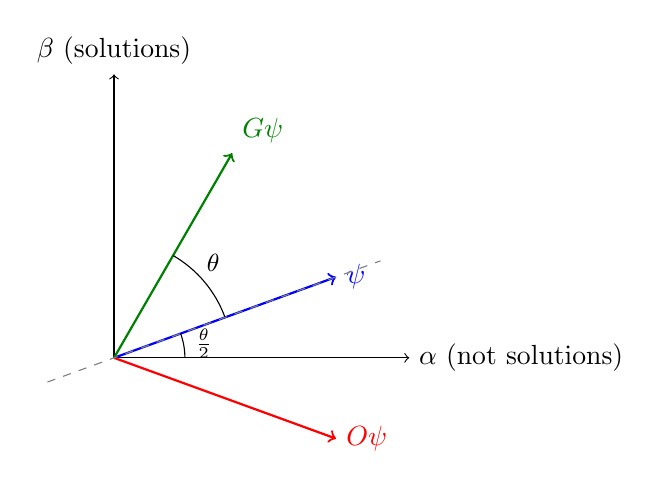
\begin{tikzpicture}[scale=3]
  \draw[->] (0,0)--(1.25,0) node[right]{$\ket\alpha$ (not solutions)};
  \draw[->] (0,0)--(0,1.2) node[above]{$\ket\beta$ (solutions)};
  \draw[->,thick,blue] (0,0)--({cos(20)},{sin(20)}) node[right]{$\ket\psi$};
  \draw[->,thick,red] (0,0)--({cos(-20)},{sin(-20)}) node[right]{$O\ket\psi$};
  \draw[->,thick,green!50!black] (0,0)--({cos(60)},{sin(60)}) node[above right]{$G\ket\psi$};
  \draw (0.3,0) arc (0:20:0.3); \node at (0.38,0.06) {\small$\frac\theta2$};
  \draw ({0.5*cos(20)},{0.5*sin(20)}) arc (20:60:0.5); \node at (0.42,0.4) {\small$\theta$};
  \draw[dashed,gray] ({-0.3*cos(20)},{-0.3*sin(20)})--({1.2*cos(20)},{1.2*sin(20)});
\end{tikzpicture}
\caption{Geometric picture of one Grover iteration. The oracle reflects $\ket\psi$ about $\ket\alpha$, and the operator $2\proj\psi-I$ reflects the result about $\ket\psi$ (dashed). The net effect is a rotation by $\theta$ towards the solutions.}
\label{fig:grover}
\end{figure}

\section{Number of iterations}
\paragraph{Example: $N=4$, $M=1$.} $\sin\frac\theta2=\frac12$, so $\frac\theta2=30^\circ$ and $\theta=60^\circ$. After a single iteration the state is at the angle $3\theta/2=90^\circ$, exactly along
$\ket\beta$. One query is enough to find the solution with certainty. A classical search needs on average $2.25$ queries if the last element is inferred without checking ($\frac14\cdot1+\frac14\cdot2+\frac12\cdot3$),
or $2.5$ if all elements are checked in a random order until the solution is found.

\paragraph{General case.} We want $(2k+1)\theta/2$ to be as close as possible to $\pi/2$. Since $\frac\pi2-\frac\theta2=\arccos\sqrt{M/N}$, the optimal number of iterations is the integer closest to
\begin{equation}
  k_{\rm opt}=\frac{\arccos\sqrt{M/N}}\theta.
\end{equation}
This requires knowing the number of solutions $M$. If we iterate too long, the state rotates past $\ket\beta$ and the success probability decreases again: \cref{eq:groverprob} is periodic in $k$
(``souffl\'e problem''). Since the final state is within an angle $\theta/2$ of $\ket\beta$, the probability of success is at least $\cos^2(\theta/2)=1-M/N$.

The algorithm works best when $M\ll N$. Then, using $\sin\theta=2\sin\frac\theta2\cos\frac\theta2$,
\begin{equation}
  \theta\approx\sin\theta=2\sqrt{\frac MN\left(1-\frac MN\right)}\approx2\sqrt{\frac MN},
\end{equation}
and the number of iterations is
\begin{equation}
  k\approx\frac\pi{2\theta}\approx\frac\pi4\sqrt{\frac NM}\sim\sqrt N.
\end{equation}
This is the square-root efficiency of Grover's algorithm. For $N=10^6$ and $M=1$, about $785$ iterations instead of $5\times10^5$ classical checks.

\paragraph{Unknown $M$.} If $M$ is unknown, one can choose $k$ at random in $[0,m)$ for increasing $m=1,\lambda,\lambda^2,\dots$ (Boyer, Brassard, Høyer, Tapp 1998), which still finds a solution in
$\order(\sqrt{N/M})$ expected queries. Alternatively, \emph{quantum counting} estimates $\theta$, and therefore $M$, by phase estimation of the eigenvalues $\e^{\pm\ii\theta}$ of $G$ (\cref{ch:shor}).

\section{Optimality}
\begin{theorem}[Bennett, Bernstein, Brassard, Vazirani \cite{BBBV1997}]
Any quantum algorithm that finds a marked element among $N$ with probability at least $1/2$ must query the oracle $\Omega(\sqrt N)$ times.
\end{theorem}
\begin{proof}[Idea of the proof (hybrid argument)]
Let $\ket{\psi_k}$ be the state after $k$ queries when no element is marked, and $\ket{\psi_k^w}$ when $w$ is marked. Each query can move the state by at most $2|a_w|$, where $a_w$ is the amplitude on
$\ket w$: $\norm{\psi_k^w-\psi_k}\le\sum_{j<k}2|a_{w,j}|$. Summing over $w$ and using Cauchy--Schwarz and $\sum_w|a_{w,j}|^2=1$, $\sum_w\norm{\psi_k^w-\psi_k}^2\le4k^2$. But to identify $w$ with high
probability, each $\ket{\psi_k^w}$ must be far from the common state $\ket{\psi_k}$, which requires $\sum_w\norm{\psi_k^w-\psi_k}^2=\Omega(N)$. Hence $k=\Omega(\sqrt N)$.
\end{proof}
Grover's algorithm is therefore optimal: for \emph{unstructured} search, quantum computers give only a quadratic speed-up. Applied to an exponentially large search space $N=2^n$, it reduces $2^n$ to $2^{n/2}$,
which is still exponential. NP-complete problems are not expected to become easy.

\section{Amplitude amplification}
Grover's algorithm generalizes: if an algorithm $\mathcal A$ (any circuit) produces a ``good'' outcome with probability $p$, then the operator $Q=-\mathcal AS_0\mathcal A^{-1}S_{\rm good}$, where $S_0$ and
$S_{\rm good}$ flip the sign of $\ket0$ and of the good states, amplifies the success probability to $\approx1$ in $\order(1/\sqrt p)$ applications, instead of the $\order(1/p)$ repetitions needed classically
(Brassard, Høyer, Mosca, Tapp 2002). Grover is the special case $\mathcal A=H^{\otimes n}$, $p=M/N$. Amplitude amplification gives quadratic speed-ups for many problems, including Monte Carlo estimation (amplitude estimation).

\section{Implementation for $N=4$}
For two qubits and the marked element $w=11$, the phase oracle is simply the CZ gate. The diffusion operator, up to a global phase $-1$, is $H^{\otimes2}(X\otimes X)\,\mathrm{CZ}\,(X\otimes X)H^{\otimes2}$, since
$(X\otimes X)\mathrm{CZ}(X\otimes X)=\diag(-1,1,1,1)=-(2\proj{00}-I)$.
\begin{center}
\begin{quantikz}
\lstick{$\ket0$} & \gate{H} & \ctrl{1}\gategroup[2,steps=1,style={dashed,rounded corners,inner sep=2pt},label style={label position=below,anchor=north,yshift=-0.2cm}]{oracle} & \gate{H} & \gate{X} & \ctrl{1} & \gate{X} & \gate{H} & \meter{}\\
\lstick{$\ket0$} & \gate{H} & \control{} & \gate{H} & \gate{X} & \control{} & \gate{X} & \gate{H} & \meter{}
\end{quantikz}
\end{center}
\begin{lstlisting}
from qiskit import QuantumCircuit
from qiskit.quantum_info import Statevector

qc = QuantumCircuit(2)
qc.h([0, 1])
qc.cz(0, 1)                         # oracle marking |11>
qc.h([0, 1]); qc.x([0, 1])          # diffusion operator
qc.cz(0, 1)
qc.x([0, 1]); qc.h([0, 1])
print(Statevector(qc).probabilities_dict())   # {'11': 1.0}
\end{lstlisting}
For larger $n$, the conditional phase shift $2\proj0-I$ requires a multi-controlled $Z$ gate on $n$ qubits, which is decomposed into $\order(n)$ Toffoli gates with ancillas. The library function
\texttt{qiskit.circuit.library.grover\_operator} builds $G$ from any oracle circuit. On present hardware, the depth of the multi-controlled gates limits useful demonstrations to a few qubits.

\section{Exercises}
\begin{exercise}
Show that for $N=8$, $M=1$, the optimal number of iterations is 2, and compute the success probability. (Answer: $\sin^2(5\theta/2)$ with $\sin(\theta/2)=1/\sqrt8$, i.e.\ $\approx0.945$.)
\end{exercise}
\begin{exercise}
Show that for $M=N/4$ a single Grover iteration finds a solution with certainty, and that for $M=N/2$ Grover's algorithm does not help at all. What is the classical success probability with one query in each case?
\end{exercise}
\begin{exercise}
Show that $G$ has eigenvalues $\e^{\pm\ii\theta}$ in the $(\ket\alpha,\ket\beta)$ plane, with eigenvectors $(\ket\alpha\pm\ii\ket\beta)/\sqrt2$.
\end{exercise}
